\chapter{Practical Operation} 
\begin{figure}[!h]
 \centering
 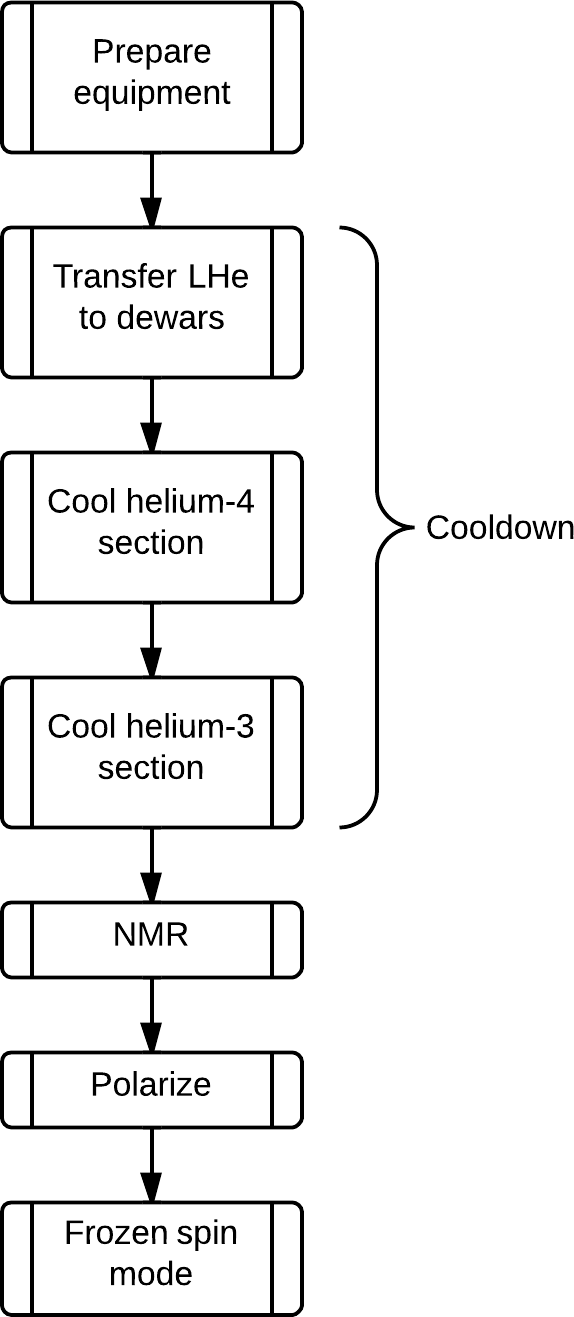
\includegraphics[scale=.24]{./img/cooldown-overview-flowchart.png}
 % cooldown-overview-flowchart.png: 102x490 pixel, 100dpi, 2.59x12.45 cm, bb=0 0 73 353
 \caption{Practical steps to polarize target material with HiFrost.}
 \label{fig:cooldown-overview-flowchart}
\end{figure}


\section{Cooldown}
\subsection{Prep}
Before LHe is ordered, the system must be verified to be in working order.  Go down the checklist found in Appendix \ref{appendix}, reporting any issues to the senior cooldown scientist.

\textbf{This step is not optional}: the rest of this operational procedure assumes all prep work is successfully completed and equipment bugs are worked out.  See walkthroughs for specifics tasks in Chapter \ref{procedures}.

\subsection{Dewar Filling}
The 500LD and 100LD are filled initally before cooling down the fridge.  Generally, it is up to the user whether to fill the magnet now or after dilution.

The 250LD has a main flow port, the pressurization port and the pressure release port.  Each of these ports has an accompanying valve.

The 500LD has an entrance port (used for filling LHe and inserting the level probe), a main flow port (outgoing LHe), a pressurization port and a pressure relief port.  Only the pressurization port and pressure relief ports have accompanying valves.

\subsubsection{500LD Fill}
\begin{enumerate}
 \item Check 250LD level using the procedure in Section \ref{procedure:check-lhe-level}.
 \item Place correct Goddard fittings on the 250LD and/or the UTL.
 \item Blow out UTL (TODO find out if UTL has flow valve) with helium gas.
 \item $[$\textbf{initial 500LD fill only}$]$ Purge the 500LD with helium gas by hooking up the pressurization line, closing the main flow valve, opening the pressure release valve and putting 5 pounds of pressure on the 500LD for about 10 minutes.  Remove the pressurization line.%for some godforsaken reason square brackets have to be in math mode to not ruin enumerated lists
 \item Open main flow valve on 500LD to vent pressure (if any), then open pressurization valve making sure the pressurization port is not pointed at anyone.
 \item Release the 250LD pressure from the main flow valve and close the pressure relief valve.  Slowly lower the correct end (TODO find if UTL is symmetric) of the UTL down into the 250LD about 30 cm or until helium gas is blowing out the 500LD end.  Then, lower the 500LD end in as far as it can go, while continuing to slowly lower the 250LD side at a rate of about 2 cm/s.  A cold plume should be coming out of the 500LD.  Check that no gas is escaping through the Goddard fittings on either dewar (if it is, replace fitting o-rings).
 \item Hook up the pressurization line to the 250LD pressurization port using the procedure in Section \ref{procedure:attach-pressurization-line} and open the pressurization valve.  There should now be 2 PSI on the 250LD.
 \item Periodically measure the 250LD level using the procedure in Section \ref{procedure:check-lhe-level}.  When it is empty, stop flow from the pressurization cylinder regulator and disconnect the pressurization line.
 \item Simultaneously raise both sides of the UTL out of the dewars and hang it on the wall to warm up.
 \item Bung the 500LD port where the UTL was, close the 500LD pressurization valve, and leave open the pressure relief valve.
 \item On the 250LD, open the pressure release valve and close the main flow and pressurization valves.
 \item Recover the Goddard fittings from the 250LD and bring it back to the weigh area.  Record the final weight on the log sheet.
\end{enumerate}

\subsubsection{Initial 100LD Fill}

The 100LD has an entrance port, a main flow port, an exhaust port and a pressure relief port.  The exhaust and pressure relief ports have accompanying valves.

\begin{enumerate}
 \item Purge the 500TL with helium gas.  Make sure the flow valve is open.
 \item Make sure the correct Goddard fittings are on the 500LD and/or 500TL.
 \item Make sure the 100TL is in the 100LD and the blue magnet valve on the WTL is closed.
 \item Open the 100LD exhaust valve, close the pressure release valve and bung the main flow valve.
 \item Remove the bung from the WTL by the pump station area.
 \item Hook up the helium gas line in the GV to the 100LD exhaust port and pressurize to 2 PSI.
 \item Verify there is a positive pressure on the WTL by the pump station.  Increase the helium cylinder pressure if necessary.  Wait 10 minutes for the 100LD, 100TL and WTL to purge.
 \item Close the 500TL flow valve and stop purging it.
 \item Vent the 500LD through the pressurization port.
 \item Open the 500LD main flow port.
 \item Close the 500LD pressurization and pressure relief valves.
 \item Slowly lower the 500LD about 30 cm until helium gas starts flowing out.  It may need to go further in first, depending on how full the 500LD is.
 \item Watch the gas plume coming out of the end of the 500TL.  Slowly lower the 500TL in the 500LD at a rate of 1cm/s until the plume looks like a blowtorch, then immediately insert into the WTL and tighten.
 \item \textbf{Immediately remove the pressurization line from the 100LD exhaust port and open the 100LD pressure relief valve.} Verify gas is coming out the exhaust and make sure the exhaust is pointing towards the center of the room and not at personnel (the plume will quickly grow).
 \item Slowly lower the 500TL all the way down into the 500LD and tighten the Goddard fitting.  Use the heat gun if the Goddard fitting freezes before the 500TL is completely in.
 \item Hook up the pressurization line to the 500LD pressurization port using the procedure in Section \ref{procedure:attach-pressurization-line} and open the 500LD pressurization valve.
 \item Turn on the 100LD level probe and watch the monitor for the level to increase.
 \item When the 100LD is full, close the 500LD pressurization valve and remove the pressurization line.  Then vent the 500LD through the pressurization port and open the 500LD pressure relief valve.
 \item Close the 500TL flow valve.
 \item Close the 100TL exhaust valve.
\end{enumerate}

\subsubsection{100LD Fill During Run}

\subsection{Cool \hef{} Section}
\subsection{Cool \het{} Section}
\subsection{Dilution}

\section{Polarization}

\section{NMR}

\section{Frozen Spin}
\blindtext
